\documentclass{article}

\usepackage{fullpage}
\usepackage{url}
\usepackage{bbm}
\usepackage{graphicx}
\usepackage{amsmath}
\usepackage{physics}
\usepackage{mathtools}
\usepackage{bbold}
\usepackage{slashed}
\usepackage{pxfonts}
\usepackage{multicol}
\usepackage{mathptmx}
\usepackage{simplewick}

\DeclareMathOperator{\erfi}{erfi}
\newcommand{\R}{\ensuremath{\mathbb{R}}}
\newcommand{\C}{\ensuremath{\mathbb{C}}}

\title{Quantum Mechanics II Excercise 6}
\author{Idan Stark}
\date{\today}

\begin{document}
\maketitle

\section{}

\section{Compelx Scalar Field}
In this section we consider the free complex scalar field:
\begin{equation}
    \mathcal{L} = \partial^\mu\varphi^*\partial_\mu\varphi - m^2 \varphi^*\varphi
\end{equation}
Where $m$ is a real constant.
\subsection{Equation of Motion}
We can find the EOM for $\varphi$ using Euler-Lagrange and treating $\varphi$ and $\varphi^*$ as seperate degrees of freedom. To find the equation for the $\varphi$ DOF, we use the EL equation for $\varphi^*$:
\begin{equation}
    \frac{\partial \mathcal{L}}{\partial\varphi^*} = -m^2\varphi
    \qquad
    \partial^\mu \frac{\partial \mathcal{L}}{\partial\left(\partial^\mu \varphi^*\right)} = \partial^\mu\partial_\mu\ = \Box \varphi
\end{equation}
Which gives:
\begin{equation}
\label{eq:varphi-eom}
    \left(\Box - m^2\right)\varphi = 0
\end{equation}
And to find the EOM for $\varphi^*$ we simply conjugate the equation:
\begin{equation}
    \left(\Box - m^2\right)\varphi^* = 0
\end{equation}
The solution to there equations can be written in mode expansion:
\begin{equation}
    \varphi(x) = \int \frac{d^3k}{(2\pi)^3}\frac{1}{\sqrt{2\omega_k}}\left(
        a_k e^{-ikx} + b_k^\dagger e^{ikx}
    \right)
\end{equation}
Where $k^0 = \omega_k = \sqrt{\vec{k} + m^2}$ and in the exponents $kx = k^0t - \vec{k}\cdot\vec{x}$. To see that it solves, we notice that:
\begin{equation}
    \Box e^{\pm ikx} = \partial^\mu\partial_\mu e^{\pm ikx} = p^\mu p_\mu e^{\pm ikx} = m^2 e^{\pm ikx}
\end{equation}
Plugging the solution into the EOM in equation \ref{eq:varphi-eom}:
\begin{equation}
    \left(\Box - m^2\right)\int \frac{d^3k}{(2\pi)^3}\frac{1}{\sqrt{2\omega_k}}\left(
        a_k e^{-ikx} + b_k^\dagger e^{ikx}
    \right) = 
    \left(m^2 - m^2\right)\int \frac{d^3k}{(2\pi)^3}\frac{1}{\sqrt{2\omega_k}}\left(
        a_k e^{-ikx} + b_k^\dagger e^{ikx}
    \right) = 0
\end{equation}
The solution for $\varphi^*$ is then, of course:
\begin{equation}
    \varphi^*(x) = \int \frac{d^3k}{(2\pi)^3}\frac{1}{\sqrt{2\omega_k}}\left(
        a_k^\dagger e^{ikx} + b_k e^{-ikx}
    \right)
\end{equation}
\subsection{Correlation Functions without Interaction}
Now, still without interaction, let us look at the correlation functions between $\varphi$ and $\varphi^*$:
\begin{equation}
    \ket{0}T\varphi(x)\varphi^*(y)\ket(0)
    \qquad
    \ket{0}T\varphi(x)\varphi(y)\ket(0)
    \qquad
    \ket{0}T\varphi^*(x)\varphi^*(y)\ket(0)
\end{equation}
Using the conjugation relations
\begin{equation}
    \left[a_k, a_p^\dagger\right] = \left[b_k, b_p^\dagger\right] = (2\pi)^3\delta^{(3)}(\vec{k} - \vec{p})
\end{equation}
with all other conjugation relations among $a_k, b_k, a_k^\dagger, b_k^\dagger$ vanishing, and the definition of the ground state
\begin{equation}
    a_k \ket{0} = b_k \ket{0} = 0
\end{equation}
Starting from the correlation function of $\varphi$ with $\varphi^*$, we open the time ordering operator:
\begin{equation}
    T\varphi(x)\varphi^*(y) = \Theta(x^0 - y^0)\varphi(x)\varphi^*(y) + \Theta(y^0 - x^0)\varphi^*(y)\varphi(x)
\end{equation}
Pluggin this into the correlation function $\bra{0}T\varphi(x)\varphi^*(y)\ket{0}$, each term gives a double k-space integral containing a combination of creationg and annihilation operators. For instance, the first expression gives:
\begin{equation}
\begin{gathered}
    \varphi(x)\varphi^*(y) = \int \frac{d^3k}{(2\pi)^3}\frac{1}{\sqrt{2\omega_k}}\left(
        a_k e^{-ikx} + b_k^\dagger e^{ikx}
    \right) \int \frac{d^3p}{(2\pi)^3}\frac{1}{\sqrt{2\omega_p}}\left(
        a_p^\dagger e^{ipy} + b_k e^{-ipy}
    \right) = \\ =
    \int \frac{d^3k}{(2\pi)^3}\frac{d^3p}{(2\pi)^3}\frac{1}{2\sqrt{\omega_k\omega_p}}\left[
        a_ka_p^\dagger e^{-i(kx - py)} +
        a_k b_k e^{-i(kx + py)} +
        b_k^\dagger a_p^\dagger e^{i(kx + py)} +
        b_k^\dagger b_k e^{i(kx - py)}
    \right]
\end{gathered}
\end{equation}
When applied to the ground state on both sides, the only terms that survive are those that have a creation operator on the right and annihilation operator on the left. In this case it's the first term $a_ka_p^\dagger$:
\begin{equation}
    \bra{0}\varphi(x)\varphi^*(y)\ket{0} = \int \frac{d^3k}{(2\pi)^3}\frac{d^3p}{(2\pi)^3}\frac{1}{2\sqrt{\omega_k\omega_p}}e^{-i(kx - py)}
    \bra{0}a_ka_p^\dagger\ket{0}
\end{equation}
Since $\bra{0}a_p^\dagger a_k\ket{0} = 0$, we can substract it in the integral to get:
\begin{equation}
    \bra{0}\varphi(x)\varphi^*(y)\ket{0} = \int \frac{d^3k}{(2\pi)^3}\frac{d^3p}{(2\pi)^3}\frac{1}{2\sqrt{\omega_k\omega_p}}e^{-i(kx - py)}
    \bra{0}\left[a_k, a_p^\dagger\right]\ket{0}
\end{equation}
And using the commutation relations:
\begin{equation}
    \bra{0}\varphi(x)\varphi^*(y)\ket{0} = \int \frac{d^3k}{(2\pi)^3}\frac{d^3p}{(2\pi)^3}\frac{1}{2\sqrt{\omega_k\omega_p}}e^{-i(kx - py)}
    (2\pi)^3\delta^{(3)}(\vec{k} - \vec{p}) = 
    \int \frac{d^3k}{(2\pi)^3}\frac{1}{2\omega_k}e^{-ik(x - y)}
\end{equation}
The other term will be the same, only to get there the surviving term will include $b_kb_p^\dagger$ and the result will have the opposite exponent:
\begin{equation}
    \bra{0}\varphi^*(y)\varphi(x)\ket{0} = 
    \int \frac{d^3k}{(2\pi)^3}\frac{1}{2\omega_k}e^{-ik(y - x)}
\end{equation}
In total, we get:
\begin{equation}
    \bra{0}T\varphi(x)\varphi^*(y)\ket{0} = \Theta(x^0 - y^0)\int \frac{d^3k}{(2\pi)^3}\frac{1}{2\omega_k}e^{-ik(x - y)} + \Theta(y^0 - x^0)\int \frac{d^3k}{(2\pi)^3}\frac{1}{2\omega_k}e^{-ik(y - x)}
\end{equation}
As we saw in class, this can be written using the Redisue theorem, as the small $\varepsilon$ limit of the complex four k-space integral:
\begin{equation}
    \Theta(x^0)\int \frac{d^3k}{(2\pi)^3}\frac{1}{2\omega_k}e^{-ikx} + \Theta(- x^0)\int \frac{d^3k}{(2\pi)^3}\frac{1}{2\omega_k}e^{ikx} = 
    \lim_{\varepsilon \rightarrow 0^{+}}\int \frac{d^4k}{(2\pi)^4}\frac{ie^{-ikx}}{k^2 - m^2 + i\varepsilon}
\end{equation}
This is because the spatial $k$ integral can be seperated from the $k^0$ integral, leaving the spatial integral similar to the above result while the $k^0$ integral is performed over the half circle contours above or below the real axis, depending on the value of $x^0$. For each contour there is a single pole at $k^0 = \pm \left(\omega_k - i\varepsilon\right)$. Solving for the residue at each pole and plugging back gives the two Heaviside functions and the opposite signes in the exponent.
\newline
Now let us turn to the other two correlation functions. In these cases, the only surviving terms are $a_k b_k^\dagger$ for the $\varphi\varphi$ case and $b_k a_k^\dagger$ for the $\varphi^*\varphi^*$ case. Using the same trick by substracting the opposite product, we get the commutators $[a_k, b_k^\dagger]$ and $[b_k, a_k^\dagger]$ respectively, which are both zero, and so the total correlation function is zero in both cases:
\begin{equation}
\begin{gathered}
    \bra{0}\varphi(x)\varphi(y)\ket{0} = \bra{0}\int \frac{d^3k}{(2\pi)^3}\frac{1}{\sqrt{2\omega_k}}\left(
        a_k e^{-ikx} + b_k^\dagger e^{ikx}
    \right) \int \frac{d^3p}{(2\pi)^3}\frac{1}{\sqrt{2\omega_p}}\left(
        a_p e^{-ipy} + b_p^\dagger e^{ipy}
    \right)\ket{0} = \\ =
    \int \frac{d^3k}{(2\pi)^3}\frac{d^3p}{(2\pi)^3}\frac{1}{2\sqrt{\omega_k\omega_p}} e^{-i(kx - py)} \bra{0}a_k b_p^\dagger\ket{0} = \\ =
    \int \frac{d^3k}{(2\pi)^3}\frac{d^3p}{(2\pi)^3}\frac{1}{2\sqrt{\omega_k\omega_p}} e^{-i(kx - py)} \bra{0}\left[a_k, b_p^\dagger\right]\ket{0} = 0
\end{gathered}
\end{equation}
And the same for the $\varphi^*\varphi^*$ case. to summarize, we got:
\begin{equation}
\begin{gathered}
    \bra{0}\varphi(x)\varphi(y)\ket{0} = \bra{0}\varphi^*(x)\varphi^*(y)\ket{0} = 0
    \\
    \bra{0}\varphi(x)\varphi^*(y)\ket{0} = D_F(x - y) = \lim_{\varepsilon \rightarrow 0^{+}}\int \frac{d^4k}{(2\pi)^4}\frac{ie^{-ik(x - y)}}{k^2 - m^2 + i\varepsilon}
\end{gathered}
\end{equation}
\subsection{Interactions correlation functions}
Now let us add an interaction term:
\begin{equation}
    \mathcal{L} = \partial^\mu\varphi^*\partial_\mu\varphi - m^2\varphi^*\varphi - \lambda(\varphi^*\varphi)^2
\end{equation}
Starting from the Vacuum correlation functions:
\begin{equation}
\begin{gathered}
    G_{1234}(x_1, x_2, x_3, x_4) = \bra{\Omega}T \varphi(x_1) \varphi(x_2) \varphi(x_3) \varphi(x_4) \ket{\Omega}
    \\
    G_{\bar{1}\bar{2}\bar{3}\bar{4}}(x_1, x_2, x_3, x_4) = \bra{\Omega}T \varphi^*(x_1) \varphi^*(x_2) \varphi^*(x_3) \varphi^*(x_4) \ket{\Omega}
    \\
    G_{12\bar{3}\bar{4}}(x_1, x_2, x_3, x_4) = \bra{\Omega}T \varphi(x_1) \varphi(x_2) \varphi^*(x_3) \varphi^*(x_4) \ket{\Omega}
\end{gathered}
\end{equation}
Using the result from before and assuming the generalization of Wick's theorem to complex scalar fields:
\begin{equation}
    \contraction{}{\varphi(x)}{}{\varphi^*(y)}\varphi(x)\varphi^*(y) = D_F(x - y)
    \qquad
    \contraction{}{\varphi(x)}{}{\varphi(y)}\varphi(x)\varphi(y) =
    \contraction{}{\varphi^*(x)}{}{\varphi^*(y)}\varphi^*(x)\varphi^*(y) = 0
\end{equation}
Let us apply this to the above correlation functions up to order of $\lambda$. In zeroth order, since the fields can only contract with themselves, both $G_{1234}^{(0)}$ and $G_{\bar{1}\bar{2}\bar{3}\bar{4}}^{(0)}$ vanish:
\begin{equation}
\begin{gathered}
    G_{1234}^{(0)}(x_1, x_2, x_3, x_4) = \bra{0}T \varphi(x_1) \varphi(x_2) \varphi(x_3) \varphi(x_4) \ket{0} = \\ =
    \contraction{}{\varphi(x_1)}{}{\varphi(x_2)}
    \contraction{\varphi(x_1)\varphi(x_2)}{\varphi(x_3)}{}{\varphi(x_4)}
    \varphi(x_1) \varphi(x_2)\varphi(x_3) \varphi(x_4) +
    \contraction{}{\varphi(x_1)}{\varphi(x_2)}{\varphi(x_3)}
    \contraction[2ex]{\varphi(x_1)}{\varphi(x_2)}{\varphi(x_3)}{\varphi(x_4)}
    \varphi(x_1) \varphi(x_2)\varphi(x_3) \varphi(x_4) +
    \contraction[2ex]{}{\varphi(x_1)}{\varphi(x_2)\varphi(x_3)}{\varphi(x_4)}
    \contraction{\varphi(x_1)}{\varphi(x_2)}{}{\varphi(x_3)}
    \varphi(x_1) \varphi(x_2)\varphi(x_3) \varphi(x_4) = 0
    \\ \\
    G_{\bar{1}\bar{2}\bar{3}\bar{4}}(x_1, x_2, x_3, x_4) = \bra{0}T \varphi^*(x_1) \varphi^*(x_2) \varphi^*(x_3) \varphi^*(x_4) \ket{0} = \\ =
    \contraction{}{\varphi^*(x_1)}{}{\varphi^*(x_2)}
    \contraction{\varphi^*(x_1)\varphi^*(x_2)}{\varphi^*(x_3)}{}{\varphi^*(x_4)}
    \varphi^*(x_1) \varphi^*(x_2)\varphi^*(x_3) \varphi^*(x_4) +
    \contraction{}{\varphi^*(x_1)}{\varphi^*(x_2)}{\varphi^*(x_3)}
    \contraction[2ex]{\varphi^*(x_1)}{\varphi^*(x_2)}{\varphi^*(x_3)}{\varphi^*(x_4)}
    \varphi^*(x_1) \varphi^*(x_2)\varphi^*(x_3) \varphi^*(x_4) +
    \contraction[2ex]{}{\varphi^*(x_1)}{\varphi^*(x_2)\varphi^*(x_3)}{\varphi^*(x_4)}
    \contraction{\varphi^*(x_1)}{\varphi^*(x_2)}{}{\varphi^*(x_3)}
    \varphi^*(x_1) \varphi^*(x_2)\varphi^*(x_3) \varphi^*(x_4) = 0
\end{gathered}
\end{equation}
This will actually happen for all orders, since in any additional interaction term there are added two $\varphi$ factors and two $\varphi^*$ factors. Any contraction of such factors still leaves two pairs of $\varphi$ for the $G_{1234}$ case and two pairs of $\varphi^*$ for the $G_{\bar{1}\bar{2}\bar{3}\bar{4}}$ case. Those pairs will have to contract with eachother, making the entire term vanish. So, for any order ot $\lambda$:
\begin{equation}
    G_{1234} = G_{\bar{1}\bar{2}\bar{3}\bar{4}} = 0
\end{equation}
Now let us look at $G_{12\bar{3}\bar{4}}$:
\begin{equation}
\begin{gathered}
    G_{12\bar{3}\bar{4}}^{(0)} = \bra{0}T \varphi(x_1) \varphi(x_2) \varphi^*(x_3) \varphi^*(x_4) \ket{0} = \\ =
    \contraction{}{\varphi(x_1)}{}{\varphi(x_2)}
    \contraction{\varphi(x_1)\varphi(x_2)}{\varphi^*(x_3)}{}{\varphi^*(x_4)}
    \varphi(x_1) \varphi(x_2)\varphi^*(x_3) \varphi^*(x_4) +
    \contraction{}{\varphi(x_1)}{\varphi(x_2)}{\varphi^*(x_3)}
    \contraction[2ex]{\varphi(x_1)}{\varphi(x_2)}{\varphi^*(x_3)}{\varphi^*(x_4)}
    \varphi(x_1) \varphi(x_2)\varphi^*(x_3) \varphi^*(x_4) +
    \contraction[2ex]{}{\varphi(x_1)}{\varphi(x_2)\varphi^*(x_3)}{\varphi^*(x_4)}
    \contraction{\varphi(x_1)}{\varphi(x_2)}{}{\varphi^*(x_3)}
    \varphi(x_1) \varphi(x_2)\varphi^*(x_3) \varphi^*(x_4) = \\ =
    D_F(x_1 - x_3)D_F(x_2 - x_4) + D_F(x_1 - x_4)D_F(x_2 - x_3)
\end{gathered}
\end{equation}
These are the two non-connected Feynman diagrams:
\begin{figure}[h]
    \centering
    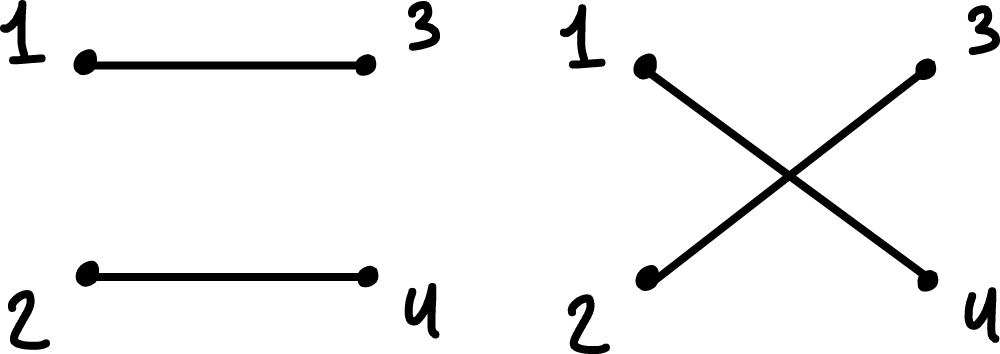
\includegraphics[width=0.5\textwidth]{Notewise-Untitled 2025-12-30-20260202133627.png}
\end{figure}
Next, let us continue to first order in $\lambda$:
\begin{equation}
    G_{12\bar{3}\bar{4}}^{(1)} = -i\lambda \int d^4z \bra{0}T \varphi(x_1) \varphi(x_2) \varphi^*(x_3) \varphi^*(x_4) \varphi^*(z) \varphi^*(z) \varphi(z)\varphi(z) \ket{0}
\end{equation}
The only possible, non-vanishing, tree-level - meaning each of the external fields is contracted to a $z$ field - contraction for this term is:
\begin{equation}
\begin{gathered}
    \bra{0}T \varphi(x_1) \varphi(x_2) \varphi^*(x_3) \varphi^*(x_4) \varphi^*(z) \varphi^*(z) \varphi(z)\varphi(z) \ket{0} =
    \contraction{}{\varphi(x_1)}{\varphi(x_2) \varphi^*(x_3) \varphi^*(x_4)}{\varphi^*(z)}
    \contraction[2ex]{\varphi(x_1)}{\varphi(x_2)}{\varphi^*(x_3) \varphi^*(x_4) \varphi^*(z)}{\varphi^*(z)}
    \contraction[3ex]{\varphi(x_1) \varphi(x_2)}{\varphi^*(x_3)}{\varphi^*(x_4)\varphi^*(z)\varphi^*(z)}{\varphi(z)}
    \contraction[4ex]{\varphi(x_1) \varphi(x_2) \varphi^*(x_3)}{ \varphi^*(x_4)}{\varphi^*(z)\varphi^*(z)\varphi(z)}{\varphi(z)}
    \varphi(x_1) \varphi(x_2) \varphi^*(x_3) \varphi^*(x_4) \varphi^*(z) \varphi^*(z) \varphi(z)\varphi(z) = \\ =
    D_F(x_1 - z)D_F(x_2 - z)D_F(z - x_3)D_F(z - x_4)
\end{gathered}
\end{equation}
Which repeats four times - twice for the $\varphi(z)$ degeneracy multiplied
by twice for the $\varphi^*(z)$ degeneracy. In total, the $O(\lambda)$ connected tree-level Feynman diagram for $G_{12\bar{3}\bar{4}}^{(1)}$ can be seen in the following diagram:
\begin{figure}[h]
    \centering
    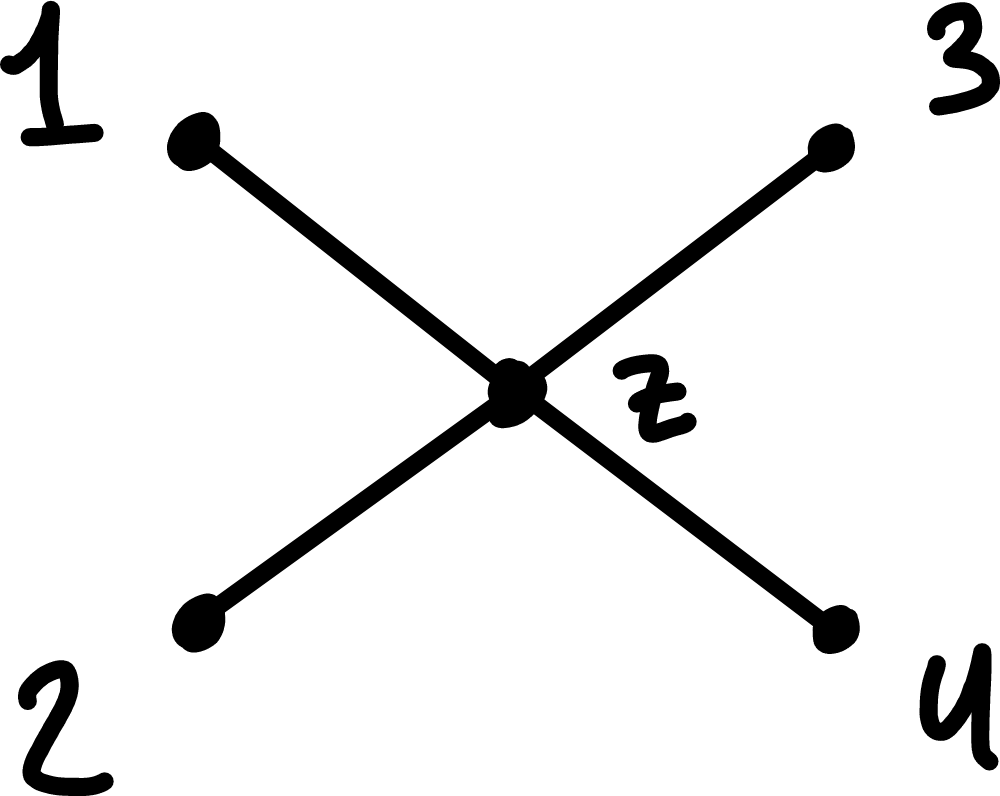
\includegraphics[width=0.5\textwidth]{Notewise-Untitled 2025-12-30-20260202134231.png}
\end{figure}
And the correlation function itself (ignoring disconnected and looping diagrams):
\begin{equation}
    G_{12\bar{3}\bar{4}} = - i4\lambda \int d^4z D_F(x_1 - z)D_F(x_2 - z)D_F(z - x_3)D_F(z - x_4)
\end{equation}

\subsection{Scattering Matrix element}
Let us now derive the scattering matrix element $M(p + p' \rightarrow k + k')$ for the particle + anti-particle pair with momenta $p$ and $p'$ to the particle + anti-particle pair with momenta $k$ and $k'$. For this, let us take the correlation function for the particle anti-particle pair $G_{12\bar{3}\bar{4}}$. Its Fourier transform is (after removing the $p, p', k, k'$ intergrals):
\begin{equation}
\begin{gathered}
    \tilde{G}_{12\bar{3}\bar{4}} = - i4\lambda \int d^4z 
    \frac{ie^{ipz}}{p^2 - m^2 + i\varepsilon}
    \frac{ie^{ikz}}{k^2 - m^2 + i\varepsilon}
    \frac{ie^{-ip'z}}{p'^2 - m^2 + i\varepsilon}
    \frac{ie^{-ik'z}}{k'^2 - m^2 + i\varepsilon} = \\ =
     - i4\lambda \int d^4z 
    \frac{e^{iz(p + k - p' - k')}}{\left(p^2 - m^2 + i\varepsilon\right)\left(k^2 - m^2 + i\varepsilon\right)\left(p'^2 - m^2 + i\varepsilon\right)\left(k'^2 - m^2 + i\varepsilon\right)} 
    = \\ = 4\lambda \delta^4(p + k - p' - k')
\end{gathered}
\end{equation}
So, we get:
\begin{equation}
    M(p + p' \rightarrow k + k') = 4\lambda
\end{equation}
\subsection{two particles to two antiparticles scattering}
As we saw in previous sections, in this theory, every contraction of a particle with a particle or a anti particle with an anti particle vanishes. The result is that the correlation function $G_{12\bar{3}\bar{4}}$ only has the option for a particle anti-particle pair to propegate into a particle anti-particle pair. This is a result of the $U(1)$ symmetry in the theory, causing a charge conservation for the total $\# particles - \# antiparticles$.

\section{Effective Theory with Dirac Fermions}
Let us consider the theory:
\begin{equation}
    \mathcal{L} = \bar{\psi}(i \slashed{\partial} - m)\psi + \frac{1}{2}\partial_\mu\phi\partial^\mu\phi - \frac{M^2}{2}\phi^2 - g\phi\bar{\psi}\psi
\end{equation}
With $\psi$ being a Dirac fermion, $\phi$ being a real scalar and $m, M, g$ being real constant parameters.

\subsection{$U(1)$ symmetry}
Let us show that the action is invariant under the global transformation:
\begin{equation}
    \psi \rightarrow e^{i\alpha}\psi
    \qquad
    \bar{\psi} \rightarrow e^{-i\alpha}\bar{\psi}
\end{equation}
For a constant $\alpha$. It's obvious to see that the second and third terms, that do not include the Dirac fermion, are unchanged. The last term:
\begin{equation}
    -g\phi\psi\bar{\psi} \rightarrow -g\phi\psi'\bar{\psi}' = -g\phi e^{i\alpha}\psi e^{-i\alpha}\bar{\psi} = -g\phi\psi e^{i\alpha} e^{-i\alpha}\bar{\psi} = -g\phi\psi\bar{\psi}
\end{equation}
And the same is true for the mass and kinetic term. Now, let us find the Noether current associated with that symmetry. To do that, let us promote $\alpha$ to a function $\alpha(x)$. Then:
\begin{equation}
\begin{gathered}
    \delta S = \delta \int d^4x \mathcal{L} = \int d^4x \mathcal{L}' - \mathcal{L} = \\ =
    \int d^4x \bar{\psi}'(i \slashed{\partial} - m)\psi' - g\phi\bar{\psi}'\psi' - \bar{\psi}(i \slashed{\partial} - m)\psi + g\phi\bar{\psi}\psi = \\ =
    \int d^4x e^{-i\alpha(x)}\bar{\psi}(i \slashed{\partial} - m)e^{i\alpha(x)}\psi - g\phi e^{-i\alpha(x)}\bar{\psi}e^{i\alpha(x)}\psi - \bar{\psi}(i \slashed{\partial} - m)\psi + g\phi\bar{\psi}\psi = \\ =
    \int d^4x e^{-i\alpha(x)}\bar{\psi}(i \slashed{\partial} - m)e^{i\alpha(x)}\psi - \bar{\psi}(i \slashed{\partial} - m)\psi = \\ =
    \int d^4x i  e^{-i\alpha(x)}(\slashed{\partial} e^{i\alpha(x)})\bar{\psi}\psi =
    - \int d^4x (\slashed{\partial}\alpha(x))\bar{\psi}\psi =
    \int d^4x \alpha(x)\slashed{\partial}\left(\bar{\psi}\psi\right)
\end{gathered}
\end{equation}
And so the conserevd current is:
\begin{equation}
    J^\mu = \partial^\mu\left(\bar{\psi}\psi\right)
\end{equation}
We can see that it is conserved from the EOM of $\psi$ and $\bar{\psi}$. To derive them, we use Euler-Lagrange:
\begin{equation}
    \frac{\partial \mathcal{L}}{\partial \bar{\psi}} = (i\slashed{\partial} - m)\psi - g\phi\psi
    \qquad
    \partial^\mu \frac{\partial \mathcal{L}}{\partial \left(\partial^\mu \bar{\psi}\right)} = 0
\end{equation}
\begin{equation}
    \left(i\slashed{\partial} - m - g\phi\right)\psi = 0
\end{equation}
* I got stuck here and ran out of time, I'm moving on to the next part.

\subsection{Vacuum correlation function}
Let us consider the time-ordered vacuum correlation function
\begin{equation}
    G(x_1, x_2; y_1, y_2) = \bra{\Omega}T\psi(x_1)\psi(x_2)\bar{\psi}(x_3)\bar{\psi}(x_4)\ket{\Omega}
\end{equation}
Up to second order in $g$, we get contributions that include two vertices $z$ and $w$ with a scalar propegator:
\begin{equation}
\begin{gathered}
    G(x_1, x_2; y_1, y_2)^{(2)} = -g^2 \int d^4z d^4w D_F(z - w) [
        S_F(x_1 - z) S_F(y_1 - z) S_F(x_2 - w) S_F(y_2 - w) - \\ -
        S_F(x_1 - z) S_F(y_2 - z) S_F(x_2 - w) S_F(y_1 - w)
    ]
\end{gathered}
\end{equation}
Where the minus sign comes from the Grassman property of the fermions switching positions during the permutation.
\begin{figure}[h]
    \centering
    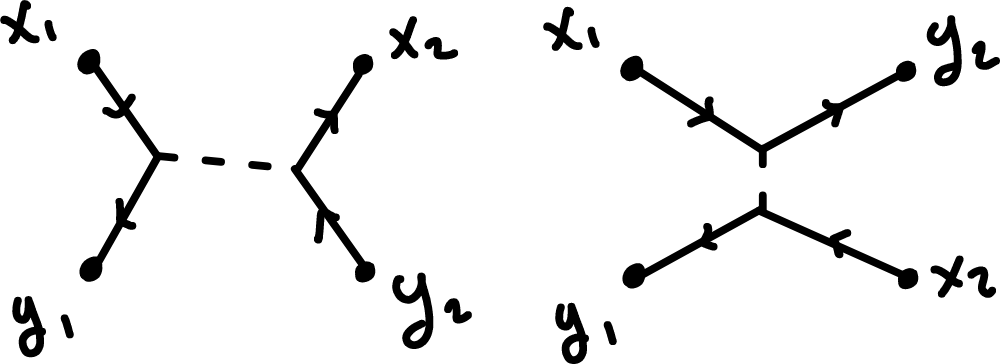
\includegraphics[width=0.5\textwidth]{Notewise-Untitled 2025-12-30-20260202133829.png}
\end{figure}
\subsection{Deriving and Effective Theory}
For a very large $M$, we can find an effective theory for $\psi$ by solving the EL equation for $\phi$ order by order in $1/M^2$. The E-L equation for $\phi$ is:
\begin{equation}
    \frac{\partial \mathcal{L}}{\partial \phi} = -M^2 \phi - g\psi\bar{\psi}
    \qquad
    \partial^\mu \frac{\partial \mathcal{L}}{\partial\left(\partial^\mu \phi\right)} = \Box \phi
\end{equation}
\begin{equation}
    \left(\Box + M^2\right)\phi = -g\psi\bar{\psi}
\end{equation}
Dividing by $M^2$ and ngelecting the derivaive terms as they have mass units and are much smaller then $M$, we get the first order approximation:
\begin{equation}
    \phi = -\frac{g}{M^2}\psi\bar{\psi}
\end{equation}
Plugging that back into the Lagrangian, we get:
\begin{equation}
    \mathcal{L} = \bar{\psi}\left(i\slashed{\partial} - m\right)\psi - \frac{g^2}{M^2}\left(\bar{\psi}\psi\right)^2
\end{equation}
Where the second and third terms in the Lagrangian were dropped because they were of order $1/M^4$ and the sign flipped for th last term when we switched the order of $\psi$ and $\bar{\psi}$ because of their Grassman properties.
\subsection{Correlation function, again}
Now we can calcualte the correlation function $G(x_1, x_2; y_1, y_2)$ from the effective theory. Using Wick's theorem up to first order in $c = -\frac{g^2}{M^2}$:
\begin{equation}
\begin{gathered}
    G_{eff}(x_1, x_2; y_1, y_2)^{(1)} = \bra{0}T\psi(x_1)\psi(x_2)\bar{\psi}(y_1)\bar{\psi}(y_2)\bar{\psi}(z)\psi(z)\bar{\psi}(z)\psi(z)\ket{0} = \\ =
    \contraction[0.5ex]{}{\psi(x_1)}{\psi(x_2)\bar{\psi}(y_1)\bar{\psi}(y_2)}{\bar{\psi}(z)}
    \contraction[2ex]{\psi(x_1)}{\psi(x_2)}{\bar{\psi}(y_1)\bar{\psi}(y_2)\bar{\psi}(z)\psi(z)}{\bar{\psi}(z)}
    \contraction{\psi(x_1)\psi(x_2)}{\bar{\psi}(y_1)}{\bar{\psi}(y_2)\bar{\psi}(z)}{\psi(z)}
    \contraction[1.5ex]{\psi(x_1)\psi(x_2)\bar{\psi}(y_1)}{\bar{\psi}(y_2)}{\bar{\psi}(z)\psi(z)\bar{\psi}(z)}{\psi(z)}
    \psi(x_1)\psi(x_2)\bar{\psi}(y_1)\bar{\psi}(y_2)\bar{\psi}(z)\psi(z)\bar{\psi}(z)\psi(z)
    -
    \contraction[0.5ex]{}{\psi(x_1)}{\psi(x_2)\bar{\psi}(y_1)\bar{\psi}(y_2)}{\bar{\psi}(z)}
    \contraction[2ex]{\psi(x_1)}{\psi(x_2)}{\bar{\psi}(y_1)\bar{\psi}(y_2)\bar{\psi}(z)\psi(z)}{\bar{\psi}(z)}
    \contraction{\psi(x_1)\psi(x_2)}{\bar{\psi}(y_1)}{\bar{\psi}(y_2)\bar{\psi}(z)\psi(z)\bar{\psi}(z)}{\psi(z)}
    \contraction[1.5ex]{\psi(x_1)\psi(x_2)\bar{\psi}(y_1)}{\bar{\psi}(y_2)}{\bar{\psi}(z)}{\psi(z)}
    \psi(x_1)\psi(x_2)\bar{\psi}(y_1)\bar{\psi}(y_2)\bar{\psi}(z)\psi(z)\bar{\psi}(z)\psi(z)
\end{gathered}
\end{equation}
Where the minus sign again comes from the Grassman property. This gives:
\begin{equation}
    G_{eff}(x_1, x_2; y_1, y_2) = -i2c \int d^4z 
        S_F(x_1 - z)S_F(x_2 - z)S_F(z - y_1)S_F(z - y_2)
\end{equation}

\subsection{Comparing the two results}
Let us now compare the results in the original and effective theories. To do that, let us integrate over $w$ in the original expression. For each of the two terms in the integral, there are three contributions related to $w$. For the first term, $D_F(z - w)S_F(x_2 - w)S_F(y_2 - w)$ and for the second term $D_F(z - w)S_F(x_2 - w)S_F(y_1 - w)$ For each of these terms, propegator give an exponential (while the rest of the propegator is independent to $w$) with the factor of the momentum. In total we will get:
\begin{equation}
\begin{gathered}
    G = \left[\begin{matrix}
        not \ related \\ to \ w
    \end{matrix}\right]
    \int d^4w e^{-iw(-q + p_1 + p_2)} + e^{-iw(-q + p_2 + p_2)} = \left[\begin{matrix}
        not \ related \\ to \ w
    \end{matrix}\right]\left[
        \delta^4(p_1 + p_2 - q) + \delta^4(p_2 + p_2 - q)
    \right]
\end{gathered}
\end{equation}
Where $p_i$ are the momenta for $x_i$ and $q$ is the momentum for the internal propeagtor. Now, the integral in $D_F(z - w)$ is simple. We already used the $w$ part of the exponential there, so the remaining integral is:
\begin{equation}
\begin{gathered}
    D_F(z - w) = \int \frac{d^4q}{(2\pi)^4}\frac{ie^{-iqz}}{q^2 - M^2 + i\epsilon}\left[
        \delta^4(p_1 + p_2 - q) + \delta^4(p_2 + p_2 - q)
    \right] = \\ = \frac{ie^{-i(p_1 + p_2)z}}{(p_1 + p_2)^2 - M^2 + i\epsilon} + \frac{ie^{-i(p_2 + p_2)z}}{(p_2 + p_2)^2 - M^2 + i\epsilon}
\end{gathered}
\end{equation}
* Ran out of time - the conecpt is pretty simple from here on. This is almost the expression needed for the comparison. We just need to expand in powers of $1/M^2$ to get the terms in the effective theory.
\end{document}